		\subsection{General Remarks}		
		\textcolor{blue}{\textbf{Gradient of a scalar field}}: Directs towards steepest rise, Zeigt richtung steilsten Anstieg.
		
		can be applied to a \textbf{gradient field}$\Rightarrow$ gives a \textbf{vector field}
		
		
		\textcolor{blue}{\textbf{Divergence of a vector field}}: Gives the tendencie of a vector field, to flow away from a point.
		
		$\operatorname{div}\vec F(\vec r) = q(\vec r) \begin{cases}
			> 0, & \text{source, quelle}\\
			= 0, & \text{source free}\\
			< 0, & \text{sink, senke}
		\end{cases}$
		
		can be applied to a \textbf{vector field} $\Rightarrow$ gives a \textbf{scalare field}
		
		\textcolor{blue}{\textbf{Curl, Rotation}} of a vector field: tendency to rotate around a point. The rotation of a vector field is a vector field of pseudo vectors. Describes the local curl density of a vector field.		
		
		can be applied to a \textbf{vector field}$\Rightarrow$ gives a \textbf{vector field}

		
		\begin{align}
			\text{Nabla operator:}\quad \nabla \: \mathrm{oder} \: \vec \nabla = \left (\frac\partial{\partial
			x_1},\ldots, \frac\partial{\partial x_n}\right)
		\end{align}
		\begin{align}
		\text{Laplace operator:}\quad \laplace \: \mathrm{oder} \: \vec \laplace = \left (\frac{\partial^2}{\partial
			x_1^2},\ldots, \frac{\partial^2}{\partial x_n^2}\right)
		\end{align}		
		\begin{align}
		 \text{Scalar function:}\quad f = f(x,y,z)
		\end{align}

		\begin{align}
		\text{vector field:}	\quad \vec F = \begin{pmatrix} F_1 \\ F_2 \\ F_3 \end{pmatrix}
		\end{align}
		
		\begin{align}
		\text{Vector product in cartesian coordinates:}\quad\vec{a}\times\vec{b} = \begin{vmatrix}
		\textbf{i} & \textbf{j} & \textbf{k} \\ a_1 & a_2 & a_3 \\ b_1 & b_2 & b_3\\ \end{vmatrix} =
		\begin{pmatrix}a_1 \\ a_2 \\ a_3\end{pmatrix} \times
		\begin{pmatrix}b_1 \\ b_2 \\ b_3 \end{pmatrix} = \begin{pmatrix} a_2b_3 - a_3b_2
		\\ a_3b_1 - a_1b_3 \\ a_1b_2 - a_2b_1 \end{pmatrix}
		\end{align}
			
\renewcommand{\arraystretch}{2}		
\begin{center}



		\begin{tabular}{llllll}
			\hline
			Function & &Nabla & &Differential form & Note \\
			\hline
			$\operatorname{grad}(f)$ &=& 
			$\nabla f$ &=&
			 $\dfrac{{\partial f}}{{\partial x}} +
			\dfrac{{\partial f}}{{\partial y}} + \dfrac{{\partial f}}{{\partial z}} = 
			\begin{pmatrix} \dfrac{\partial f}{\partial x}, \quad\dfrac{\partial f}{\partial
				y}, \quad \dfrac{\partial f}{\partial z} \end{pmatrix}$&\\	
			\hline 
			$\operatorname{div}\vec F$ &=& 
			$\nabla \cdot \vec F$&=&
			$\dfrac{\partial}{\partial x_1}F_1 + \dfrac{\partial}{\partial x_2}F_2+ \dfrac{\partial}{\partial x_3}F_3$&\\
			\hline
			$\mathbf{\operatorname{rot}}\,\vec F$ &=& 
			$\nabla\times \vec F$ &=& 
			$\begin{pmatrix} \dfrac{\partial}{\partial x} \\ \dfrac{\partial}{\partial y} \\
				\dfrac{\partial}{\partial z} \end{pmatrix} \times \begin{pmatrix} F_x\\ F_y\\ F_z
			\end{pmatrix} = \begin{pmatrix} \dfrac{\partial F_z}{\partial y} - \dfrac{\partial
				F_y}{\partial z} \\ \dfrac{\partial F_x}{\partial z} - \dfrac{\partial
				F_z}{\partial x} \\ \dfrac{\partial F_y}{\partial x} - \dfrac{\partial
				F_x}{\partial y} \end{pmatrix}$&
			$\mathbf{\wedge = \times} \newline$\\ 
			&&
			&=&
			$ \left (\dfrac{\partial F_y}{\partial x} - \dfrac{\partial F_x}{\partial y}\right )\vec e_z$ & 2 Dimensional\\
			\hline
		\end{tabular}
\end{center}
\renewcommand{\arraystretch}{1.2}				


	
	\subsection{Calculation rules (Bronstein p.731)}
	Vector filds : $\vec F$, $\vec G$ 
	
	Scalar fields: $U$, $V$
	
	constant, constant field: $c, \vec{c}$
	
\renewcommand{\arraystretch}{2}					
	\begin{tabularx}{\textwidth}{|X|X|}
		\hline
		$\operatorname{grad}\,c=\vec{0}$ & $\operatorname{grad}\,(c\cdot u)=c\cdot\operatorname{grad}\,U$    \\
		\hline
		$\operatorname{grad}\,(U+V)=\operatorname{grad}\,U+\operatorname{grad}\,V$ &
		$\operatorname{grad}\,(U\,V) = U\ \operatorname{grad}\,V + V\ \operatorname{grad}\,U$\\
		\hline
		$\label{eqn:ProduktregelEinesGradientMitPotenzen}
		\operatorname{grad}\,(U^n) = n\, U^{n-1}\ \operatorname{grad}\,U \text{ f�r } n\neq 0$&
		$\operatorname{rot}(\operatorname{grad}U)=\nabla \times (\nabla U) = 0$ \\
		\hline\hline
		$\operatorname{div}\,\vec{c}=\vec{0}$&
		$\operatorname{div}\,(c\cdot \vec{F})=c\cdot\operatorname{div}\,\vec{F}$ \\
		\hline
		$\operatorname{div}\,(\vec{F}+\vec{G})=\operatorname{div}\,\vec{F}+\operatorname{div}\,\vec{G}$ &
		$\operatorname{div}\,(U\,\vec{F}) = U\ \operatorname{div}\,\vec{F} + \vec{F}\cdot \operatorname{grad}\,U$\\		
		\hline
		$\operatorname{div}\,(\vec{F} \times\vec{G})=\vec{G}\cdot \operatorname{rot}\,\vec{F} - \vec{F}\operatorname{rot}\,\vec{G}$ &
		$\operatorname{div}(\operatorname{rot}\vec{F}) = \nabla \cdot (\nabla \times\vec F) = 0$\\
		\hline\hline
		
		$\operatorname{rot}\,(\vec{F}+\vec{G})=\operatorname{rot}\,\vec{F}+\operatorname{rot}\,\vec{G}$ &
		$\operatorname{rot}\,(c \vec{F})=c\operatorname{rot}\,\vec{F}$ \\
		\hline
		$\operatorname{rot}\,(U\,\vec{F}) = U\ \operatorname{rot}\,\vec{F} + \operatorname{grad}\,U \times \vec{F}$&
		$\operatorname{rot}\,(\vec{F} \times\vec{G}) =\newline (\vec{G}\cdot \operatorname{grad})\,\vec{F} - (\vec{F}\cdot \operatorname{grad})\,\vec{G} + \vec{F}\operatorname{div}\vec{G} - \vec{G}\operatorname{div}\,\vec{F}$
		
		
		
		
		\\
		\hline\hline
		$	\operatorname{rot}(\operatorname{rot}\vec{F}) = \operatorname{grad}(\operatorname{div}\vec{F}) -\Delta \vec{F}$&\\
		\hline
		$\operatorname{grad}(UV)=U\operatorname{grad}V+V\operatorname{grad}U $ &
		$\operatorname{grad}(\vec{F}\cdot \vec{G}) = (\operatorname{grad}\vec{F})^{\operatorname t}\vec{G} + (\operatorname{grad}\vec{G})^{\operatorname t}\vec{F} $ \\
		\hline
		$	\operatorname{div}(U\vec{F})=U\operatorname{div}\vec{F}+\vec{F}\cdot\operatorname{grad}U $&
		$\operatorname{div}(\vec{F}\times \vec{G})= \vec{G} \cdot\operatorname{rot}\vec{F} -\vec{F}\cdot\operatorname{rot}\vec{G} $ \\				
		\hline
		$\operatorname{rot}(U\vec{F})= U\operatorname{rot}\vec{F}-\vec{F}\times\operatorname{grad}U\ $& 
		$\operatorname{grad}\,\varphi(U) = \dfrac{d\varphi}{dU}\operatorname{grad}\,U$
		\\
		\hline
	
		
	\end{tabularx}
\renewcommand{\arraystretch}{1.2}						

	
	\subsection{Divergence Theorem of Gauss}
	Transformation between Volume and Surface Integrals, in a vector Field $\vec{F}$.
		
	\begin{align}
		\int_V \operatorname{div} \vec{F} \; \mathrm dV = 
		\int_V \nabla\cdot \vec{F} \; \mathrm dV =
		\oint_{S} \vec F \cdot\vec n\; \mathrm dA
	\end{align}
	
	\subsection{Stoke's Theorem}
	Transformation between Surface and Line Integrals.	Das Kurven- oder Linienintegral eines r�umlichen Vektorfeldes $\vec F$ l�ngs einer geschlossenen Kurve $\partial F$ ist gleich dem Oberfl�chenintegral der
	Rotation von $\vec u$ �ber eine beliebige Fl�che $F$, die durch die Kurve
	$\partial F$ berandet wird:
	
	\begin{align}
		\int_{F} \operatorname{rot} \vec u \cdot d \vec A =
		\int_{F} \nabla \times \vec u \cdot d \vec A =
		\oint_{\partial F} \vec u \cdot d \vec r
	\end{align}
	

	\subsection{Beispiel} % Exercise Chapter 3 (a)
	
	\subsubsection{Gauss Theorem}
	kubischer W�rfel [1m, 1m, 1m] in 3d\\
	Vektorfeld: $v = v_0 (\frac{x_1}{a}, \frac{x_2}{a}, 0)^T$ mit $v_0 = 0.1 m/s$
	und $a = 1m$\\
	
	\textbf{sketch flow field in $x_1$, $x_2$-plane}\\
	
	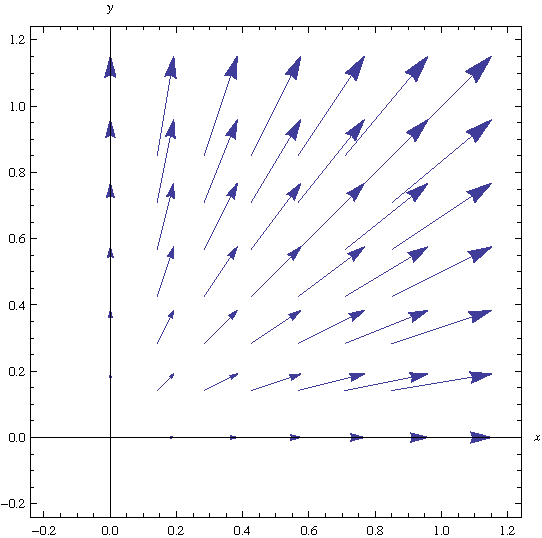
\includegraphics[scale=0.5]{images/gauss.pdf}\\ % weg mit dem figure plunder
	Vectorfield\\
	
	
	\textbf{Fluss �ber Fl�che berechnen}\\
	Fluss �ber alle Fl�chen summieren:\\
	Fl�che unten $x_1$,$x_3$ bei $x_2 = 0$:
	\begin{align}
		\oint_{S} \vec u \cdot
		\vec n\; \mathrm dA = \frac{v_0}{a} \oint_{S} \begin{pmatrix}
			x_1\\ x_2\\ 0
		\end{pmatrix} \cdot
		\begin{pmatrix}
			0\\ -1\\ 0
		\end{pmatrix} \mathrm dA = \frac{v_0}{a} \int_{0}^{1} \int_{0}^{1} x_2 \mathrm
		dx_1 \mathrm dx_3 = \frac{v_0}{a} \int_{0}^{1} \int_{0}^{1} 0 \mathrm dx_1
		\mathrm dx_3 = 0
	\end{align}
	Fl�che oben $x_1$,$x_3$ bei $x_2 = 1$:
	\begin{align}
		\oint_{S}
		\vec n\; \mathrm dA = \frac{v_0}{a} \oint_{S} \begin{pmatrix}
			x_1\\ x_2\\ 0
		\end{pmatrix} \cdot
		\begin{pmatrix}
			0\\ -1\\ 0
		\end{pmatrix} \mathrm dA = \frac{v_0}{a} \int_{0}^{1} \int_{0}^{1} x_2 \mathrm
		dx_1 \mathrm dx_3 = \frac{v_0}{a} \int_{0}^{1} \int_{0}^{1} 1 \mathrm dx_1
		\mathrm dx_3 = \frac{v_0}{a}
	\end{align}
	Fl�che hinten $x_1$,$x_2$ bei $x_3 = 1$:
	\begin{align}
		\oint_{S} \vec u \cdot
		\vec n\; \mathrm dA = \oint_{S} \frac{v_0}{a} \begin{pmatrix}
			x_1\\ x_2\\ 0
		\end{pmatrix} \cdot
		\begin{pmatrix}
			0\\ 0\\ 1
		\end{pmatrix} \mathrm dA = \int_{0}^{1} \int_{0}^{1} 0 \mathrm dx_1 \mathrm
		dx_2 = 0
	\end{align}
	Sinngem�ss f�r alle Fl�chen Durchziehen:
	\begin{align}
		I_{tot} = \frac{v_0}{a} + \frac{v_0}{a} + 0 + 0 + 0 + 0 = 2 \frac{v_0}{a}
	\end{align}
	
	Mit Gauss theorem �ber Fl�che (einfacher):
	\begin{align}
		\int_V \nabla \vec u \; \mathrm dV = \int_V \nabla \begin{pmatrix}
			x_1\\ x_2\\ 0
		\end{pmatrix} \; \mathrm dV = \int_{V}
		\frac{\partial x_1}{\partial x_1} + \frac{\partial x_2}{\partial x_2} +
		\frac{\partial 0}{\partial x_3} \; \mathrm dV =
		\frac{v_0}{a}
		\int_{0}^{1}
		\int_{0}^{1}
		\int_{0}^{1} 1 + 1 + 0 \; \mathrm dx_1 \mathrm dx_2 \mathrm dx_3 = 2
		\frac{v_0}{a}
	\end{align}
